\documentclass[12pt,a4paper]{article}
\usepackage[T1]{fontenc}
\usepackage[utf8]{inputenc}
\usepackage[italian]{babel}
\usepackage{geometry}
\usepackage{graphicx}
\usepackage{wrapfig}
\usepackage{csquotes}
\usepackage{makecell}
\usepackage{comment}

\geometry{a4paper,left=2cm,right=2cm}


\begin{document}
	\begin{titlepage}
		\centering
		\vspace*{\fill}
		{\scshape\LARGE Università degli Studi di Verona \par}
		\vspace{1.5cm}
		
\includegraphics[scale=0.5]{images/univr_logo.png}
		\vspace{1.5cm}\\
		\line(1,0){250} \\
		{\huge\bfseries Online Library\par}
		{\Large\bfseries Documentazione al prototipo \par}
		\line(1,0){250} \\
		\vspace{0.5cm}
		{\Large Magdalena M. Solitro\par}
		\vspace{2cm}
		
		\vspace{5cm}
		\vspace*{\fill}
		% Bottom of the page
		{}
		{\large \today\par}
	\end{titlepage}
	\newpage
	\tableofcontents
	\newpage
	\section{Introduzione}
	L'obiettivo di questo progetto era quello di sviluppare un software che simulasse un'applicazione online di e-commerce per una libreria.\\Questa relazione costituisce la documentazione del prototipo, in cui spiegheremo l'utilizzo del software e descriveremo le scelte progettuali e implementative adottate.
	\section{Requisiti}
	I requisiti del progetto sono stati specificati nella consegna, che riportiamo integralmente di seguito:
	\begin{quotation}
		\textit{Si vuole progettare un sistema informatico per gestire gli acquisti on-line di una libreria.
		\paragraph{}Per ogni libro si memorizza il titolo, l’autore o gli autori, la casa editrice, l’anno di pubblicazione, il codice ISBN (identificativo), il genere, il prezzo ed una breve descrizione.\\ Gli utenti possono visualizzare le classifiche di vendita che sono organizzate per genere (novità, narrativa, ragazzi, ...) e vengono aggiornate ogni settimana. Per ogni posizione della classifica si indica da quante settimana il libro è in quella posizione.
		\paragraph{}Il sistema memorizza gli ordini degli utenti. Gli utenti possono essere registrati o meno. Per gli utenti si memorizzano nome, cognome, indirizzo, CAP, città, numero di telefono ed email. Ogni utente registrato accede con email e password ed ha associata una LibroCard per la raccolta punti. Ogni LibroCard ha un numero identificativo, una data di emissione e il totale dei punti raccolti. Gli utenti registrati possono specificare uno o più indirizzi di spedizione diversi da quello di residenza.
		\paragraph{}Ogni libro ha associato il numero di punti che vengono caricati sulle LibroCard in caso di acquisto da parte di utenti registrati.
		\paragraph{}Per ogni ordine si memorizzano il codice (univoco), la data, i libri che lo compongono, l’utente che lo ha effettuato, il costo totale, il tipo di pagamento (carta di credito, paypal o contrassegno) e il saldo punti se l’utente è registrato
		\paragraph{}Il sistema deve permettere agli utenti registrati di accedere al loro profilo, modificare i dati anagrafici, verificare il saldo punti e lo stato dei loro ordini. Ogni utente registrato può vedere tutti gli ordini che ha effettuato nel tempo con il totale dei punti accumulati per ogni ordine.
		Gli utenti non registrati possono accedere agli ordini cha hanno effettuato tramite il codice dell’ordine.
		\paragraph{}I responsabili della libreria devono poter verificare lo stato degli ordini, e il saldo punti delle LibroCard degli utenti registrati.
		Inoltre, i responsabili della libreria sono responsabili dell’inserimento dei dati relativi ai libri che si possono ordinare e dell’aggiornamento delle classifiche.
		Tutti gli utenti sono opportunamente autenticati dal sistema per poter accedere alle funzionalità di loro competenza.}
	\end{quotation}
	\section{UML}
	\subsection{Use Cases}
	In questa sezione verranno presentate alcune schede dei casi d'uso principali.\\Quali casi d'uso? visualizzazione tutte librocard (employee), inserimento nuovo libro (employee)\vspace{10px}, inserimento nuovo dipendente\\
	% ridefinisco lo spazio tra righe
	\renewcommand{\arraystretch}{2.0}
	% aumento lo spazio tra colonne
	\setlength{\tabcolsep}{15pt}
	\begin{tabular}{| l | l |}
		\hline
		\textbf{ID} & UC1: Registrazione utente\\
		\hline
		\textbf{Attori} & Utente non registrato\\
		\hline
		\textbf{Precondizioni} & \\
		\hline
		\textbf{Sequenza} & \makecell[l]{
		\\1) L'utente clicca sul pulsante \texttt{Sign Up} e viene portato nella pa-\\gina di registrazione\vspace{5px}\\
		2) L'utente inserisce i propri dati anagrafici, le informazioni di \\contatto e una password negli appositi campi\vspace{5px}\\
		3) L'utente clicca sul pulsante \texttt{Sign Up}\\
		\quad\quad3.a) Se l'utente risulta essere già registrato, presenta un mes-\\\quad\quad saggio di errore e rifiuta la registrazione\\
		\quad\quad3.b) Se l'utente non riempie alcuni campi, presenta un messag-\\\quad\quad gio di errore e rifiuta la registrazione\\
		\quad\quad3.c) Se nel campo di controllo della password l'utente inserisce\\\quad\quad una password diversa, presenta un messaggio di errore e rifiu-\\\quad\quad ta la registrazione\vspace{5px}\\}\\
		\hline
		\textbf{Postcondizioni} & L'utente è stato correttamente inserito nel database\\
		\hline
	\end{tabular}
	\begin{tabular}{|l|l|}
		\hline
		\textbf{ID} & UC2: Creazione di un ordine\\
		\hline
		\textbf{Attori} & Utente registrato\\
		\hline
		\textbf{Precondizioni} & \makecell[l]{\\1. L'utente deve aver effettuato il log in\vspace{5px}\\2. Il carrello dell'utente deve avere almeno un articolo\vspace{5px}\\}\\
		\hline
		\textbf{Sequenza} & \makecell[l]{\\1) Dalla pagina del carrello, l'utente clicca il pulsante \texttt{Check Out}\\
		\quad\quad1.a Se il carrello è vuoto, viene presentato un messaggio d'erro-\\\quad\quad re che impedisce di procedere all'acquisto\vspace{5px}\\
		2) L'utente seleziona un metodo di pagamento\vspace{5px}\\
		3) L'utente sceglie l'indirizzo di spedizione, che può essere quello di \\domicilio o un altro indirizzo \vspace{5px}\\
		\quad\quad 3.a) Se l'utente sceglie un indirizzo diverso da quello del domici-\\\quad\quad lio, allora deve specificare l'indirizzo nel campo apposito\vspace{5px}\\
		4) L'utente clicca sul pulsante \texttt{Check Out}\vspace{5px}\\
		\quad\quad 4.a) Se l'utente non ha selezionato un metodo di pagamento o\\\quad\quad non ha specificato l'indirizzo alternativo, viene presentato un \\
		\quad\quad messaggio d'errore che richiede l'inserimento dei dati mancanti\vspace{5px}\\}\\
		\hline
		\textbf{Postcondizioni} & L'ordine viene confermato\\
		\hline
	\end{tabular}
	\begin{tabular}{|l|l|}
		\hline
		\textbf{ID} & UC3: Creazione di un ordine\\
		\hline
		\textbf{Attori} & Utente non registrato\\
		\hline
		\textbf{Precondizioni} & \makecell[l]{Il carrello dell'utente deve avere almeno un articolo\vspace{5px}\\}\\
		\hline
		\textbf{Sequenza} & \makecell[l]{\\1) Dalla pagina del carrello, l'utente clicca il pulsante \texttt{Check Out}\\
			\quad\quad1.a) Se il carrello è vuoto, viene presentato un messaggio d'erro-\\\quad\quad re che impedisce di procedere all'acquisto\vspace{5px}\\
			2) L'utente deve specificare: nome, cognome, metodo di pagamento,\\un indirizzo di spedizione e le informazioni di contatto nei campi ap-\\positi \vspace{5px}\\
			3) L'utente clicca sul pulsante \texttt{Check Out}\vspace{5px}\\
			\quad\quad 3.a) Se l'utente non ha inserito tutti i campi richiesti, viene pre-\\\quad\quad sentato un messaggio d'errore che impedisce di completare \\\quad\quad l'acquisto\vspace{5px}\\}\\
		\hline
		\textbf{Postcondizioni} & L'ordine viene confermato\\
		\hline
	\end{tabular}
	\vspace{20px}
	\newpage
	\begin{tabular}{|l|l|}
		\hline
		\textbf{ID} & UC4: Modifica dei dati personali\\
		\hline
		\textbf{Attori} & Utente registrato\\
		\hline
		\textbf{Precondizioni} & \makecell[l]{L'utente deve aver effettuato il log in\vspace{5px}\\}\\
		\hline
		\textbf{Sequenza} & \makecell[l]{\\1) Dalla pagina del profilo, l'utente clicca il pulsante \texttt{Modify} \\ \texttt{your data}, che porta alla pagina di modifica dei dati\vspace{5px}\\
		2) L'utente riempie esclusivamente i campi che desidera modifi-\\care\vspace{5px}\\
		3) Se l'utente clicca sul pulsante \texttt{Confirm changes}, si apre un \\messaggio che richiede la conferma della modifica:\vspace{5px}\\
		\hspace{11px} 3.1) Se l'utente clicca sul pulsante \texttt{OK} del dialog, i dati nel\\ 
		\hspace{38px}database vengono modificati e l'utente viene riportato \\
		\hspace{38px}nella pagina del profilo\vspace{5px}\\
		\hspace{11px} 3.2) Se l'utente clicca sul pulsante \texttt{Cancel}, il dialog si chiude\\
		\hspace{38px}e si resta nella pagina di modifica dei dati\vspace{5px}\\
		4) Se l'utente clicca sul pulsante \texttt{Cancel} della pagina, si apre un\\
		messaggio che richiede la conferma dell'azione:\vspace{5px}\\
		\hspace{11px} 4.1) Se l'utente clicca il pulsante \texttt{OK} del dialog, si viene ripor-\\
		\hspace{38px}tati nella pagina del profilo e i dati restano immutati\vspace{5px}\\
		\hspace{11px} 4.2) Se l'utente clicca il pulsante \texttt{Cancel} del dialog, si resta \\
		\hspace{38px} nella pagina di modifica dei dati\vspace{5px}}\\
		\hline
		\textbf{Postcondizioni} & I dati dell'utente vengono modificati, oppure restano inalterati\\
		\hline
	\end{tabular}
	\newpage
	\begin{tabular}{|l|l|}
		\hline
		\textbf{ID} & UC5: Ricerca di un ordine\\
		\hline
		\textbf{Attori} & Utente non registrato\\
		\hline
		\textbf{Precondizioni} & \\
		\hline
		\textbf{Sequenza} & \makecell[l]{\\1) Dalla \texttt{MainPage}, l'utente clicca sulla scritta \texttt{MY ORDERS} in\\alto
		a sinistra\vspace{5px}\\
		2) L'utente viene portato nella pagina di relativa al traccia-\\mento degli ordini\vspace{5px}\\
		3) L'utente inserisce nel campo apposito il codice univoco \\dell'ordine che desidera visualizzare\vspace{5px}\\
		4) L'utente clicca sul pulsante di ricerca \texttt{Search}:\vspace{5px}\\
		\hspace{15px}4.1) Se il codice corrisponde effettivamente a un ordine re-\\
		\hspace{38px}gistrato nel database, si visualizzano le relative infor-\\
		\hspace{38px}mazioni\vspace{5px}\\}\\
		\hline
		\textbf{Caso d'eccezione} & \makecell[l]{\\Se il codice non corrisponde ad alcun ordine presente nel data-\\base, si apre un messaggio d'errore\vspace{5px}}\\
		\hline
		\textbf{Postcondizione} & \makecell[l]{\\L'utente visualizza le informazioni relative all'ordine se questo\\ è presente nel database.\vspace{5px}\\}\\
		\hline
	\end{tabular}
	\newpage
	\begin{tabular}{|l|l|}
		\hline
		\textbf{ID} & UC6: Aggiunta di un libro al carrello\\
		\hline
		\textbf{Attori} & Utente registrato\\
		\hline
		\textbf{Precondizioni} & L'utente deve aver effettuato il log in\\
		\hline
		\textbf{Sequenza} & \makecell[l]{\\1) Dalla \texttt{MainPage}, l'utente seleziona un libro\vspace{5px}\\
		2) L'utente viene portato nella pagina contenente tutte le infor-\\
		\hspace{15px}mazioni relative al libro\vspace{5px}\\
		3) Se l'utente desidera più di una copia di quel libro, può sele-\\
		\hspace{15px}zionare fino a dieci unità tramite lo Spinner a destra\vspace{5px}\\
		4) L'utente clicca sul pulsante \texttt{Add To Cart} per aggiungere il \\
		\hspace{15px}libro\vspace{5px}\\}\\
		\hline
		\textbf{Caso d'eccezione} & \makecell[l]{\\1) Se non ci sono più copie di quel libro, viene presentato un \\
		\hspace{15px}messaggio d'errore e il libro non viene aggiunto\vspace{5px}\\
		2) Se il libro è già presente nel carrello, viene presentato un\\
		\hspace{15px}messaggio di errore e il libro non viene aggiunto\vspace{5px}\\}\\
		\hline
		\textbf{Postcondizione} & \makecell[l]{Il libro è stato aggiunto al carrello}\\
		\hline
	\end{tabular}
	\newpage
	\subsection{Activity Diagram}
	\subsection{Class Diagram}
	\begin{figure}[h!]
		\centering
		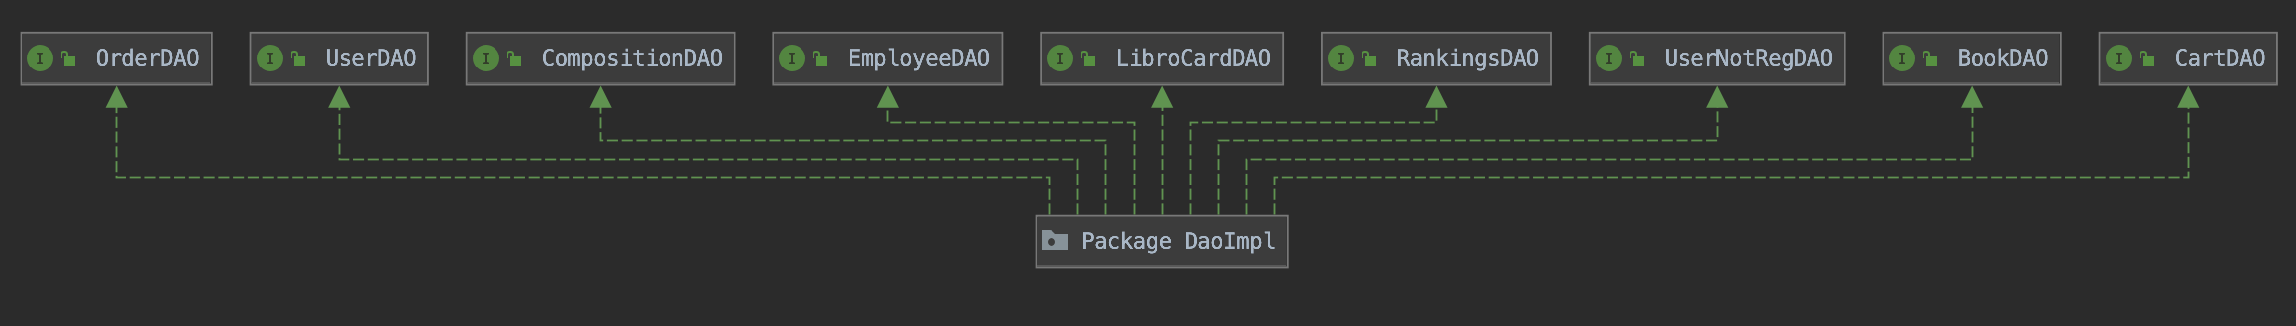
\includegraphics[scale=0.43]{images/Utils.png}
		\caption{Class Diagram per il package Utils}
	\end{figure}
	\begin{figure}[h!]
		\centering
		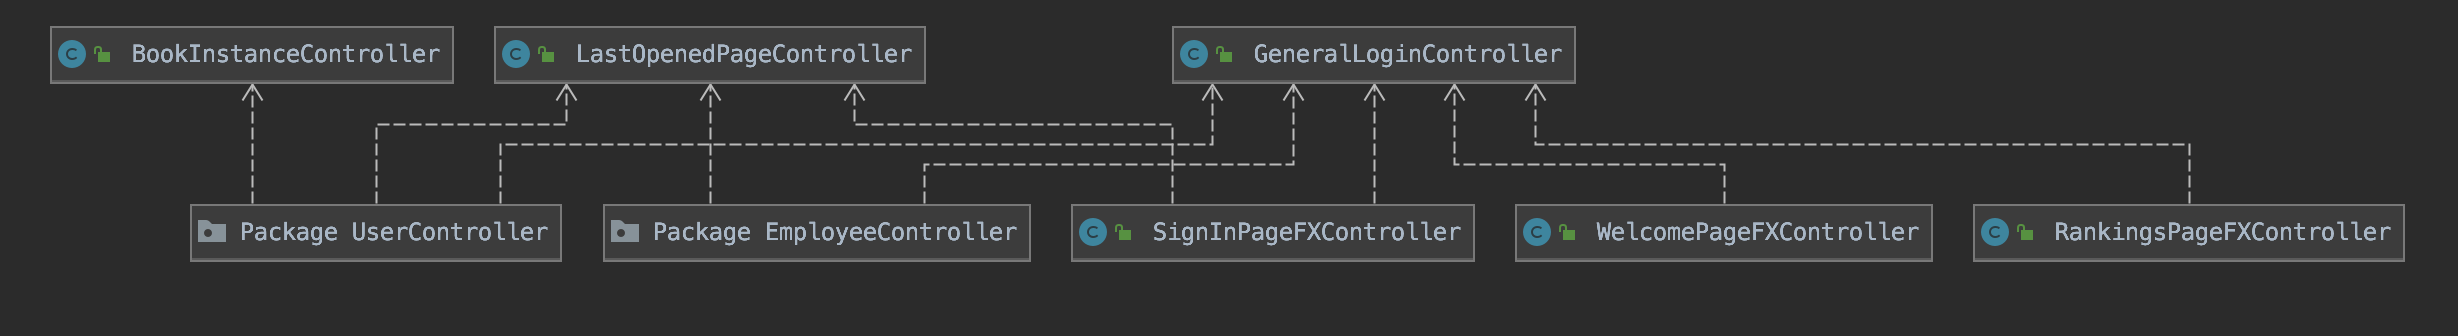
\includegraphics[scale=0.4]{images/Controller.png}
		\caption{Class Diagram per il package Controller}
	\end{figure}
	\subsection{Sequence Diagram}
	\section{Scelte progettuali}
	\subsection{Sviluppo} 
	Questo progetto è stato sviluppato principalmente Java, che costituisce un linguaggio estremamente vario e flessibile, e ancora oggi risulta essere molto diffuso nel mercato.\\Per l'interfaccia grafica ho deciso di utilizzare due strumenti: JavaFX, una libreria nativa di Java, e FXML, un linguaggio di mark-up basato su XML. \\JavaFX rappresenta un'alternativa sicuramente più ricca e versatile rispetto a Swing, che è stato invece il tool proposto a lezione: essa permette infatti di realizzare GUI molto più elaborate, grazie alla presenza di animazioni, oggetti geometrici 2D e 3D, grafici, contenuti multimediali, e altro.\\FXML, invece, è stato scelto perché permette di utilizzare un designer di interfacce grafice, Scene Builder, che rende la progettazione sicuramente più semplice e veloce. Inoltre, FXML è particolarmente adatto a interagire con JavaFX, visto che la struttura gerarchica del file rispecchia esattamente la struttura del \textit{scene graph} di JavaFX.\\
	Per stilizzare ulteriormente gli elementi dell'interfaccia grafica si è utilizzato anche CSS, che è completamente supportato sia da JavaFX, sia da FXML.
	\subsection{Metodologia di sviluppo}
	Il progetto è stato sviluppato con il supporto di Git come sistema di code versioning e di GitHub per l'hosting del repository.
	È stata seguita una metodologia di sviluppo Agile ...
	\subsection{Database}
	Fin dall'inizio, risultava evidente la necessità di mantenere i dati nel tempo: per questo motivo ho deciso di far uso di un database, sfruttando così anche le conoscenze apprese durante il corso di Database frequentato durante lo sviluppo del progetto.\\
	Dato che la gestione e l'utilizzo del database non rientravano negli obiettivi del progetto, ho scelto di utilizzare SQLite, che costituisce un RDBMS semplice, leggero e open-source.\\
	SQLite è un database engine \textit{"serverless"}, che viene quindi memorizzato interamente in locale, ed è inoltre scritto interamente in C, il che lo rende particolarmente veloce.\\
	Questo strumento presenta tuttavia anche dei limiti ... \\
	\subsubsection{Schema logico}
	
	\subsubsection{Schema relazionale}
	\subsection{MVC Pattern}
	Il funzionamento del progetto è basato sul MVC pattern, che prevede la suddivisione logica delle classi in tre componenti:
	\begin{figure}[h!]
		\centering
		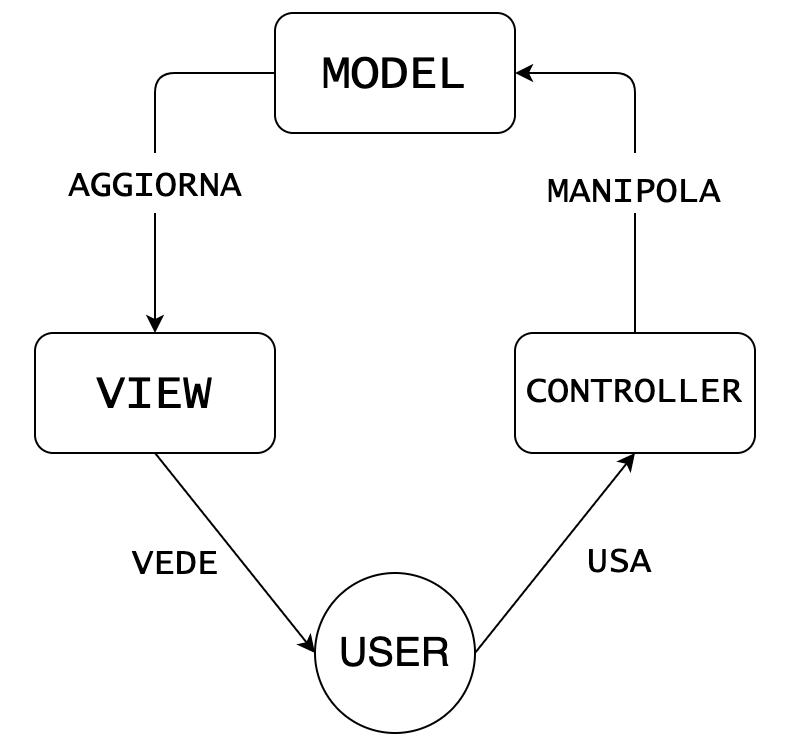
\includegraphics[scale=0.4]{images/MVCPattern.png}
	\end{figure}\\
	...
	\subsection{Singleton Pattern}
	Il \textit{Singleton Pattern} è stato utilizzato per limitare l'instanziazione di un oggetto a uno solo. In termini pratici, l'applicazione può essere usata da un solo utente alla volta, e quindi non è possibile essere loggati durante la stessa sessione come due utenti diversi. Nonostante l'applicazione simuli idealmente un sito di e-commerce, quindi un'applicazione web a cui possono accedere più utenti contemporaneamente, nella pratica è stata sviluppata come un'applicazione desktop: di conseguenza il software non è utilizzabile da più persone contemporaneamente, e questo giustifica l'utilizzo di questo design pattern.
	L'implementazione di questo pattern è stata sviluppata nella classe \texttt{GeneralLoginController}: la classe contiene l'attributo \texttt{loginInstance}, inizialmente settato a \texttt{null}, la cui funzione è memorizzare una stringa che identifica univocamente l'utente che ha eseguito il login.\\
	Quando l'utente esegue il logout, il valore della stringa torna ad essere \texttt{null}.\\
	\subsection{Observer Pattern}
	L'\textit{Observer Patter} prevede che un oggetto possa impostare una lista di "ascoltatori" (tecnicamente chiamati \textit{Observers} o \textit{Listeners}) che vengono notificati automaticamente ogni qualvolta lo stato dell'oggetto cambia. 
	Questo pattern è stato utilizzato nell'interfaccia grafica, per ottenere dei cambiamenti dinamici in risposta alle interazioni dell'utente con determinati elementi. \\Più precisamente, è stato impiegato nei seguenti contesti:
	\begin{itemize}
		\item nella \texttt{MainPage} dei clienti (registrati e non), per visualizzare i libri appartenenti a un determinato genere;
		\item nelle \texttt{RankingsPage} dei clienti e dei responsabili, per visualizzare le classifiche relative a un determinato genere;
		\item in \texttt{AllLibroCardsPage}, ovvero la pagina che consente ai responsabili della libreria di controllare le LibroCard degli utenti. In questo caso, l'interfaccia cambiava a seconda che si volesse effettaure la ricerca della LibroCard con l'e-mail dell'utente o con la cardID;
		\item in \texttt{AllOrdersPage}, ovvero la pagina che permette ai responsabili di controllare lo stato degli ordini. In questo caso, l'insieme degli ordini visualizzato cambiava in base allo stato che veniva selezionato.
	\end{itemize}
	\subsection{Data Access Object Pattern}
	Per la gestione del database ho deciso di adottare il \textit{Data Access Object Pattern}, che permette di separare l'insieme delle azioni che l'applicazione ha bisogno di eseguire sul database dal modo in cui esse sono concretamente implementate.\\
	Per ogni classe del \texttt{Model} è stata quindi definita un'interfaccia \texttt{DAO}, contenente la dichiarazione dei metodi tramite cui l'oggetto poteva interagire con il database. Ad ogni interfaccia corrisponde una classe \texttt{DaoImpl} che la implementa, sfruttando l'API di Java per l'interazione con i DBMS, JDBC, e semplici query SQL.
	\section{Validazione}
	\section{Conclusioni}
\end{document}